\documentclass[tikz]{standalone}
\usepackage{bm}
\usepackage{stix}

\definecolor{mplblue}{HTML}{1f77b4}

\tikzstyle{neuron}=[circle, draw, minimum size=0.8cm, inner sep=0pt]
\tikzstyle{box}=[rounded corners, draw, minimum width=0.8cm, minimum height=0.48cm]

\begin{document}
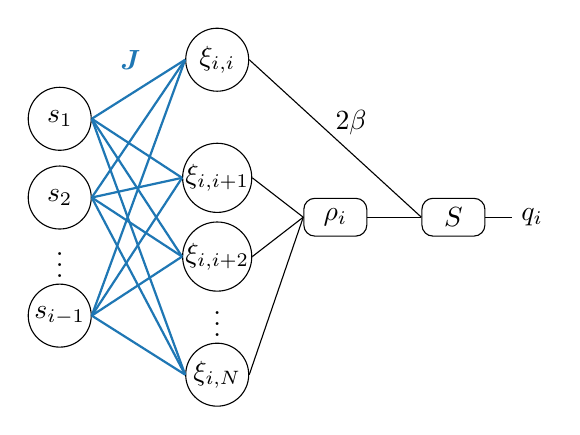
\begin{tikzpicture}[y=-1cm]

\node[neuron] (s1) at (0, 0.75) {$s_1$};
\node[neuron] (s2) at (0, 1.75) {$s_2$};
\node at (0, 2.5) {$\vdots$};
\node[neuron] (s9) at (0, 3.25) {$s_{i - 1}$};

\node[neuron] (x0) at (2, 0) {$\xi_{i, i}$};
\node[neuron] (x1) at (2, 1.5) {$\xi_{i, i + 1}$};
\node[neuron] (x2) at (2, 2.5) {$\xi_{i, i + 2}$};
\node at (2, 3.25) {$\vdots$};
\node[neuron] (x9) at (2, 4) {$\xi_{i, N}$};

\draw[mplblue, thick] (s1.east) -- (x0.west);
\draw[mplblue, thick] (s1.east) -- (x1.west);
\draw[mplblue, thick] (s1.east) -- (x2.west);
\draw[mplblue, thick] (s1.east) -- (x9.west);
\draw[mplblue, thick] (s2.east) -- (x0.west);
\draw[mplblue, thick] (s2.east) -- (x1.west);
\draw[mplblue, thick] (s2.east) -- (x2.west);
\draw[mplblue, thick] (s2.east) -- (x9.west);
\draw[mplblue, thick] (s9.east) -- (x0.west);
\draw[mplblue, thick] (s9.east) -- (x1.west);
\draw[mplblue, thick] (s9.east) -- (x2.west);
\draw[mplblue, thick] (s9.east) -- (x9.west);

\node at (0.9, 0) {\color{mplblue} $\bm{J}$};

\node[box] (rho) at (3.5, 2) {$\rho_i$};
\node[box] (S) at (5, 2) {$S$};
\node (q) at (6, 2) {$q_i$};

\draw (x1.east) -- (rho.west);
\draw (x2.east) -- (rho.west);
\draw (x9.east) -- (rho.west);

\draw (x0.east) -- (S.west);
\draw (rho.east) -- (S.west);

\draw (S.east) -- (q.west);

\node at (3.7, 0.8) {$2 \beta$};

\end{tikzpicture}
\end{document}
